\chapter{Requirements}
\label{cha:requirements}


\section{Execution environment}

I have already mentioned, that the approach taken in this work is based on
``separation  through  virtualization''.   This  section  deals  with  the
requirements to  the system  and what a  user should  be able to  do.

An \emph{execution environment} should at least meet the following points:
\begin{enumerate}
\item start new tasks
\item stop running tasks
\item list running tasks
\item query the status of tasks
\item reservation of remote resources
\item providing input data for a task
\item retrieving generated data from a finished task
\end{enumerate}

Additionally this work is  about a \emph{Xen based} execution environment,
so that  means that if a user  wants to execute an  application the system
will create a new virtual machine.

The application  need not to  be run  locally, it can  be run on  a remote
system  --- the  only requirement  is, that  the data  can  be transferred
there.  That will be the base functionality of the here designed system:

\begin{quote}
  \emph{``executing applications on remote systems using Xen instances''}
\end{quote}

\paragraph{Starting an application}

To be able to create a virtual  machine on the remote site the user has to
specify not only  the application she wants to run but  also an image that
contains the  required operating  system.  The execution  environment then
takes care of starting up the  virtual machine with the provided image and
eventually execute the application.

For later  reference to the  just created task, the  execution environment
must assign a unique identifier that can  be used by the user to manage or
query the status of that task.

\paragraph{Managing running tasks}

Given  that the user  started a  task earlier,  he may  want to  query the
status of  that task. He could  also want to abort  the task, if  he is no
longer  interested in  it. The  execution  environment gave  out a  unique
identifier with which the user now can refer to the task.

The may also be interested in an overview of tasks that he has started, so
the environment  should present  him a  list of all  his tasks  along with
their states.

\paragraph{Reserving resources}

A more  advanced usage  is the reservation  of resources in  advance. That
means a user can specify everything she  would as if she wanted to start a
new task but additionally she says  for example when the task shall start. 
The execution environments is required to meet that constraint.

\paragraph{Accessing the data}

Computational programs usually work on some input data and generate output
data of differing  amount. The system I am going to  design must offer the
user functionalities  to transfer  input data to  the virtual  machine and
output data back.

\bigskip

We have now sketched the requirements  to the environment and can now have
a look at its building blocks.

\section{Architecture}
\label{sec:architecture}

This  section  introduces  the  desired architecture  of  the  ``Xen-based
execution     environment''.      The     system    as     depicted     in
Fig.~\ref{fig:architecture}   essentially   consists   of  the   following
components:
\begin{enumerate}
  
\item some kind of a user --- that could be a real person using the system
  on  one hand  or  a script  or some  other  program such  as a  ``Calana
  Broker''        (described        in        \cite{dalheimer05agentbased,
    dalheimer06calanaprotocol}) on the other hand.
  
\item a central  managing daemon running on a Xen  \cite{xen} host or more
  concretely within \texttt{dom0}.  This part is, for instance, accessible
  through a command line, a web service or some other interface. A user in
  general  does  only   talk  directly  to  this  part   of  the  system.  
  Fig.~\ref{fig:architecture} shows this part  as the ``Xen Manager''.
  
\item the third component resides  directly on a Xen instance and provides
  several functions to the  managing daemon (``Xen instance controller''). 
  Functionalities  of this component  include: monitoring  and controlling
  the user's  application, mounting external data  locations and providing
  access to generated results.

\end{enumerate}

\begin{figure}[htbp]
  \begin{center}
%    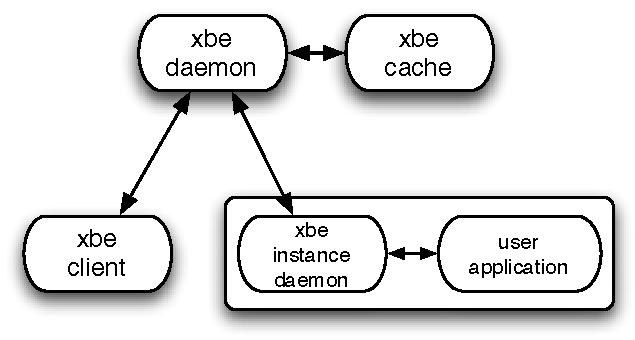
\includegraphics[height=80mm]{architecture-overview}
  \end{center}
  \caption[Architecture overview]{An overview over the conceptual
    architecture}
  \label{fig:architecture}
\end{figure}

The other parts of the figure are storage locations, such as ``image'' and
``data'' locations.   That are those sites  where a user  can store images
with applications  or data  and that  can be accessed  by the  system.

The  application images  for  instance  must be  accessible  by the  ``Xen
Manager'' to be able to boot  up a virtual machine.  Data images, used for
input to  and output from the  application, must be made  available to the
``Xen  instance  controller''.  The  ``image  cache''  can  be seen  as  a
secondary image  location, it can be  used to store images  to access them
faster (``locality of reference'', \cite{locality-principle}).

The next  section deals with  several use cases  that are of  interest for
users and administrators of this system.

\section{Use cases}

In  an  earlier   section  I  have  shortly  described,   what  the  basic
requirements to this  system are and now  I am going to show  you some use
cases and which parts of the architecture are involved in each.

The  big  picture  is  shown  in  \ref{fig:system-usecases},  it  shows  a
compendium of several possible use cases from a very high level.

\begin{figure}[htbp]
  \begin{center}
%    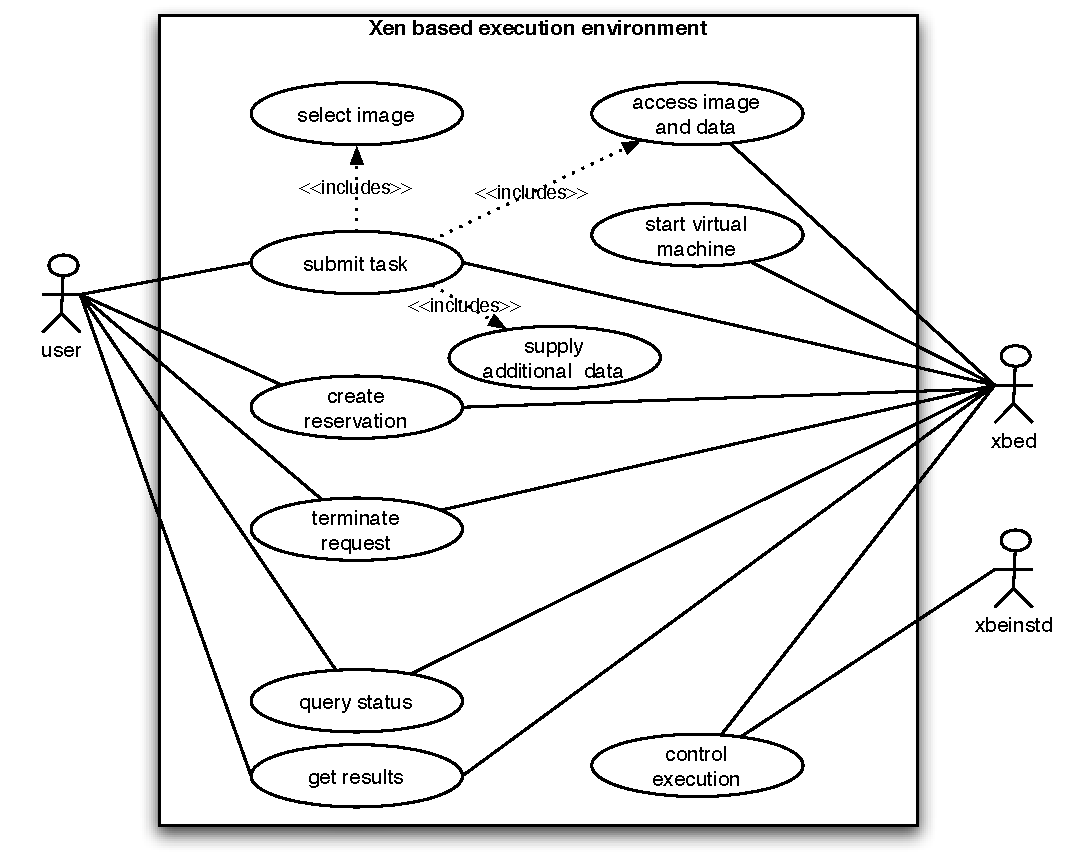
\includegraphics[width=0.9\textwidth]{system-usecase}
  \end{center}
  \caption[Use case overview]{an overview over several possible use cases}
  \label{fig:system-usecases}
\end{figure}

The use cases are split into several scenarios which can arise during that
particular  case. Now  let's go  through each  use case  step by  step and
analyze on that way where possible problems could occur.

\subsection{Use case 1: image submission}
\label{uc:1}

The  first use case  is about  the submission  of images,  that are  to be
executed on a remote host. The main  objective of this use case is how the
user can specify which image he wants to submit and eventually be run.

\subsubsection{Scenario 1.1 --- submitting a single image}

The easiest scenario  is in which the user only has  one image. This image
contains  everything: the  operating  system, the  application and  needed
input  data.  That  means  all needed  information  is within  the image.  
Figure~\ref{fig:arch-uc-1.1} shows the  relevant parts of the architecture
that are involved in this scenario.

\begin{figure}[htbp]
  \begin{center}
%    \includegraphics[height=8cm]{architecture-uc-1-1}
  \end{center}
  \caption[Architecture UC 1.1]{parts of the architecture relevant to use
    case 1.1}
  \label{fig:arch-uc-1.1}
\end{figure}

The user specifies the location (i.e. an URI) of the image and passes this
information to  the ``Xen Manager'' along  with a description  of the task
that  he desires  to execute.  The ``Xen  Manager'' will  then  attempt to
download the  image from the  specified location. 

\begin{figure}[htbp]
  \begin{center}
%    \includegraphics[height=8cm]{sequence-image-submission-1}
  \end{center}
  \caption[Sequence UC 1.1]{sequence diagram for the image submission}
  \label{fig:seq-uc-1.1}
\end{figure}

When the image  has been successfully retrieved, the  ``Xen Manager'' will
create  a  special  Xen  instance  to  run the  image.

\bigskip

\paragraph*{When will the image be started?}

The answer simply  is ``it depends''. That is because  the boot up process
takes some  time and may vary  of course.  Additionally the  image must be
transferred from some  location to the server and  that consumes even more
time. If a user wants to have some guaranty, it will be required, that
\begin{enumerate}
\item the image does already reside on the server
\item a reservation has been made
\end{enumerate}

This  particular topic is  a use  case on  its own  and will  be discussed
later.

\paragraph*{What happens if errors occur?}

Errors can occur  in each step of the  submission.  During the interactive
part (i.e. submission  of the job description) errors  may be communicated
directly back to the user.

If an error  occurs during the transfer of some image,  there is no direct
way  to tell  the user  about it.   But  the user  can check  later on  if
something went  wrong using the  unique identifier she  got.  Additionally
could there be  a notification service, to which  the user subscribes with
the unique identifier. This service could then send out messages to inform
the user.

\subsubsection{Scenario 1.2 --- submitting several images}

In the first  scenario all data had to be within  one image, this drawback
is addressed in this scenario. The components used in this scenario are
shown in Fig.~\ref{fig:arch-uc-1.2}

Along with an  image the user can specify locations  from which input data
may be retrieved  and to which generated data should  be sent --- commonly
known as staging operations. These locations can be any URI as long as the
appropriate operation (read/write) can be executed.

\begin{figure}[htbp]
  \begin{center}
%    \includegraphics[height=8cm]{architecture-uc-1-2}
  \end{center}
  \caption[Architecture UC 1.2]{parts of the architecture relevant to use
    case 1.2}
  \label{fig:arch-uc-1.2}
\end{figure}

\subsection{Use case 2: caching of images}
\label{uc:2}

Imagine a user,  who wants to execute the same  application several times. 
That would  mean he has  to submit the  same image again and  again, which
imposes a heavy load on the network connecting user and provider (i.e. the
host  on which the  Xen Manager  runs). It  is wise  to provide  a caching
mechanism, that allows the user to store his image at server-side.

The    architecture    needed    for     this    case    is    shown    in
Fig.~\ref{fig:arch-uc-caching}.

\begin{figure}[htbp]
  \begin{center}
%    \includegraphics[height=5cm]{architecture-uc-caching-1}
  \end{center}
  \caption[Architecture UC 2]{parts of the architecture relevant for caching}
  \label{fig:arch-uc-caching}
\end{figure}

\paragraph{How gets the image transferred?} There are two answers to this
question, that can be  categorized into ``active'' and ``passive'' caching
from the user's point of view.
\begin{itemize}
\item Prior to any job submission, the user (actively) transfers the image
  to the server  (Fig.~\ref{fig:seq-image-caching-1}).
  \begin{figure}[htbp]
    \begin{center}
%      \includegraphics[width=0.75\textwidth]{sequence-image-caching-1}
    \end{center}
    \caption[Image caching sequence 1]{actively caching an image}
    \label{fig:seq-image-caching-1}
  \end{figure}
  Later  on, when the  user wants  to submit  a job,  he passes  the cache
  location --- represented by a unique identifier --- to the server.
  
\item The user specifies a job description as described in use case 1. The
  Xen Manager  not only  retrieves the  image to start  the job,  but also
  stores it in the cache (Fig.~\ref{fig:seq-image-caching-2}).
  \begin{figure}[htbp]
    \begin{center}
%      \includegraphics[width=0.75\textwidth]{sequence-image-caching-2}
    \end{center}
    \caption[Image caching sequence 2]{an image gets passively cached by
      the Xen Manager}
    \label{fig:seq-image-caching-2}
  \end{figure}
\end{itemize}


\paragraph{How is the cached image referenced?} To efficiently use cached
images, it is required that the user can reference them somehow. More than
one solution is here possible, too.
\begin{itemize}
\item The user uses the unique  identifier he got when he stored the image
  in   the    cache   in   the    first   place,   this   is    shown   in
  Fig.~\ref{fig:seq-image-caching-3}.
  \begin{figure}[htbp]
    \begin{center}
%      \includegraphics[width=0.75\textwidth]{sequence-image-caching-3}
    \end{center}
    \caption[Image referencing]{retrieving a referenced image from the cache}
    \label{fig:seq-image-caching-3}
  \end{figure}
\item The user  queries the Xen Manager to give him  a descriptive list of
  all   cached   images,   that   are   accessible  by   the   user   (see
  Fig.~\ref{fig:seq-image-caching-4}).   Descriptive means here,  that the
  user is presented with some detailed information about the images.
  \begin{figure}[htbp]
    \begin{center}
%      \includegraphics[width=0.75\textwidth]{sequence-image-caching-4}
    \end{center}
    \caption[Image referencing]{retrieving a referenced image from the cache}
    \label{fig:seq-image-caching-4}
  \end{figure}
\end{itemize}

The    components   involved    in    this   scenario    are   shown    in
Fig.~\ref{fig:arch-referencing-images-1}.
\begin{figure}[htbp]
  \begin{center}
%    \includegraphics[height=5cm]{architecture-referencing-cached-images-1}
  \end{center}
  \caption{Architecture of use case 2}
  \label{fig:arch-referencing-images-1}
\end{figure}


\subsection{Use case 3: image deployment}

This use case  deals with the starting process of  images. The Xen Manager
uses the image  that the user specified and starts up  a Xen instance. The
steps  required   to  start   up  such  a   new  instance  are   shown  in
Fig.~\ref{fig:seq-image-deployment-1} and consist of:
\begin{enumerate}
\item  The instance  itself has  to be  started.
\item  During  that an  instance  controller  is  being started  ---  this
  controller  is   responsible  for  starting,   monitoring  and  stopping
  applications and several other housekeeping functionalities.
\item The Xen Manager connects to the instance controller, thus confirming
  that the instance is fully available.
\end{enumerate}

\begin{figure}[htbp]
  \begin{center}
%    \includegraphics[height=5cm]{sequence-image-deployment-1}
  \end{center}
  \caption[Image deployment sequence]{the steps required to be taken to
    start up a new instance}
  \label{fig:seq-image-deployment-1}
\end{figure}

After  successfully  connecting  from  the  Xen Manager  to  the  instance
controller, both  sides are in  the state ``instance  controllable'', that
means that:
\begin{itemize}
\item applications can be started through the controller
\item started applications can be monitored and controlled
\end{itemize}

Additionally  it   is  possible  to   retrieve  the  streams   of  started
applications.        The        architecture       as       shown       in
Fig.~\ref{fig:arch-deployment-1}   is  now   enriched   by  the   instance
controller running on a Xen instance.

\begin{figure}[htbp]
  \begin{center}
%    \includegraphics[height=5cm]{architecture-deployment-1}
  \end{center}
  \caption[Image deployment architecture]{a Xen Manager controlling three
    Xen instances}
  \label{fig:arch-deployment-1}
\end{figure}


\subsection{Use case 4: controlling and monitoring}

A  full-fledged execution  environment demands  mechanisms to  control and
monitor its activities.   At all times the user must be  able to:
\begin{itemize}
\item  query the status  of her  running application  --- the  sequence of
  actions is shown in Fig.~\ref{fig:seq-status-query-1}.
  \begin{figure}[htbp]
    \begin{center}
%      \includegraphics[height=5cm]{sequence-status-query-1}
    \end{center}
    \caption[Querying the status]{a user querying the status of his application}
    \label{fig:seq-status-query-1}
  \end{figure}
\item and  she should also be able  to abort the very  same execution (see
  Fig.~\ref{fig:seq-abort-task-1}).
  \begin{figure}[htbp]
    \begin{center}
%      \includegraphics[height=5cm]{sequence-abort-task-1}
    \end{center}
    \caption[Aborting a running task]{a user requesting the abortion of a
      running task}
    \label{fig:seq-abort-task-1}
  \end{figure}
\end{itemize}

The OGSA-BES  draft \cite{ogsa-bes} defines a  standardized description of
job states (Fig.~\ref{fig:ogsa-bes-model-1})  which can easily be extended
without breaking  components relying on the  ``non-extended'' model.  This
standard  can be used  to describe  the states  of an  application running
within a Xen instance.

\begin{figure}[htbp]
  \begin{center}
%    \includegraphics[height=5cm]{ogsa-bes-state-model-1}
  \end{center}
  \caption{The basic OGSA-BES state model}
  \label{fig:ogsa-bes-model-1}
\end{figure}


\paragraph{What, if the application is not running yet?}

Imagine a  user requesting the current  state of his  newly submitted job,
the Xen  Manager answers all  questions as best  as it can. That  means he
would       for       example       react      as       described       in
Table~\ref{tab:monitor-cases-overview}.
\begin{table}[htbp]
  \begin{center}
    \begin{tabular*}{0.9\textwidth}{p{0.4\textwidth}|p{0.4\textwidth}}
      current situation & state returned \\ \hline\hline
      image not yet available & \texttt{pending} (image loading)\\ \hline
      instance not yet started & \texttt{pending} (instance) \\ \hline
      application not yet started & \texttt{pending} (application) \\ \hline
      image could not be retrieved & \texttt{failed} (image retrieval) \\ \hline
      instance could not be started & \texttt{failed} (instance) \\ \hline
      application could not be started & \texttt{failed} (application)
    \end{tabular*}
    \caption[States returned by the Xen Manager]{States returned by the Xen Manager in several cases}
    \label{tab:monitor-cases-overview}
  \end{center}
\end{table}


\subsection{Use case 5: resource reservation}

An advanced subject is to provide advance reservation. That means that the
user  has the  possibility  to tell  the  Xen Manager,  that  he needs  an
instance for a given  time and at a specific point in  time.  Later on the
user can specify which image the Xen Manager should use.

The steps taken are presumably as follows:
\begin{enumerate}
\item The user  makes a reservation of some resource,  i.e. number of CPUs
  for a given duration --- five hours  for example --- and a point in time
  at       which      the       reservation      may       start      (see
  Fig.~\ref{fig:seq-advance-reservation-1}).
  \begin{figure}[htbp]
    \begin{center}
%      \includegraphics[width=0.75\textwidth]{sequence-advance-reservation-1}
    \end{center}
    \caption{Making a reservation}
    \label{fig:seq-advance-reservation-1}
  \end{figure}
  
\item After obtaining  a (unique) reservation ID, the  user can submit any
  job  he  likes  and  he  is  guaranteed, that  job  will  start  by  the
  reservation's start time.
  \begin{figure}[htbp]
    \begin{center}
%      \includegraphics[width=0.75\textwidth]{sequence-advance-reservation-2}
    \end{center}
    \caption{Submitting a job using a reservation}
    \label{fig:seq-advance-reservation-2}
  \end{figure}
  
\item The  Xen Manager acts as if  it was an ordinary  job submission, but
  this time he waits with starting up the instance until the start time of
  the reservation is reached.
  \begin{figure}[htbp]
    \begin{center}
%      \includegraphics[width=0.75\textwidth]{sequence-advance-reservation-3}
    \end{center}
    \caption{Starting an instance with a reservation}
    \label{fig:seq-advance-reservation-3}
  \end{figure}
\end{enumerate}

So  the  actual submission  of  an  image is  split  into  two parts,  the
reservation  part  and  the  eventual  assignment  of  an  image  to  that
reservation.

It seems  to be  very simple but  there are  some problems that  come into
mind.

\paragraph{What happens if the image is not available?}

This case can easily been run into, if the reservation shall start but the
image is not yet available. The user has to be informed about that and the
job can not be run.

One  solution  to  that  is   to  provide  the  image  before  making  any
reservations or  submissions using that  image, thus the user  makes sure,
that  the image  will be  available when  needed. Another  (less failsafe)
solution  is to  have  enough time  between  submission and  start of  the
reservation  ---  this  highly  depends  on  how fast  the  image  can  be
retrieved.

\paragraph{What if a reservation ends before the application exits}

This may  happen, since  users can not  always exactly foresee  when their
application will  end and thus  may specify a  too short duration  for the
reservation.  Ordinary batch-scheduler usually  give a little more time to
the application and stop it (i.e.  forcing it to quit) eventually.

\begin{figure}[htbp]
  \begin{center}
%    \includegraphics[width=0.75\textwidth]{sequence-advance-reservation-4}
  \end{center}
  \caption{Suspending an instance}
  \label{fig:seq-advance-reservation-4}
\end{figure}

Xen provides  the possibility  to suspend the  instance and  continuing it
later  (Fig.~\ref{fig:seq-advance-reservation-4}).  The  problems involved
with suspension of  a running instance are discussed in  the next use case
``check-pointing''.


\subsection{Use case 6: check-pointing}

In Fig.~\ref{fig:seq-advance-reservation-4} you  have seen how an instance
has been  suspended in the case  of reservation expiry  --- suspension can
also    be    used    to    provide    the   user    with    a    snapshot
\cite{distributed-snapshots} or check-pointing mechanism.

The steps taken  are essentially the same ---  suspending the instance due
to some event,  saving the state and resuming it later  --- this is called
an ``offline snapshot''.

\paragraph{What are the events?}

As        in         use        case        ``advance        reservation''
(Fig.~\ref{fig:seq-advance-reservation-4}),   one   event   may   be   the
expiration of a reservation, but there are more:

\begin{itemize}
\item the application itself triggers  an event, indicating that now would
  be a good point to do a snapshot
\item a snapshot is taken regularly by the system
\item  the user  wants to  make a  snapshot (manually  triggered)  --- for
  instance after four hours of computation.
\end{itemize}


\paragraph{Problems that can occur}

One big  problem of taking a  snapshot in this way  are active connections
(e.g.  TCP  connections) from the instance,  those cannot be  saved by the
system  and  must  therefore  be  reinitialized by  the  application  upon
resuming.

The application  does not necessarily need  to know that  the instance has
been suspended, so it  seems to it like a link or  network failure. As you
can  see, the  application  must be  able  to recover  from  that kind  of
failure.

Even worse are connections{\bf to}  the instance, since after resuming the
IP address  of the instance  may have changed.  To overcome this,  the Xen
Manager is required to assign the same address to this instance.

\subsection{Use case 7: updating existing images}

So far,  we were only interested  in how a  user is involved in  the image
execution  process.  But  what  about  an site  administrator  who has  to
administer all the cached or especially provided application images. Those
applications and  operating system distributes  need updates from  time to
time, but there could be plenty of such images residing in the database.

This problem  directly leads to  the need for  an automated task  that can
update the software components within  an image and execute a special test
case designed to confirm that everything is still working.

%%% Local Variables: 
%%% mode: latex
%%% TeX-master: "main.tex"
%%% End: 
